\documentclass[12pt]{report}
\usepackage{graphicx}

\title{\textbf{Safe driving using your android smart-phone}}
\author{
        Manu Sharma\\201351021\\Anjul Kumar Tyagi\\201352029\\Aditya Prakash\\201351010\\Yash Choubey\\201351006
		}
\date{31july,2015}
\begin{document}

\maketitle
\textbf{Abstract}\\
“In the present world we all do see the rise in road accidents and also experience that very few measures are taken for such accidents before they occur. Mobile phones especially smart phones are equipped with the efficient sensors and other features that can together form a portable device to monitor road conditions.”\textbf{[1]}\\
Imagine yourself driving blinded , yet you have no worry because there is a system which tells you exactly what to dodge any accident ahead.\\
Of course you would prefer that you hadn't had to drive at all. Years from now that may be possible. Lets not be that futuristic. Unfortunately you have to drive for now. But we will help you with all the information you need to know about the road ahead. If you live in India, you definitely need to have the knowledge we are imparting.\\
You want to know the speed breakers ahead, we got it. You want to know any other road anomalies, we got them too. We got it all. From GPS to AWS ( Advanced Warning System ), its all in your cell phone.\\
We present to you an Advanced Warning System for detecting and alarming about the road anomalies up ahead on your route. We will also collect the data from your phone about the problems you faced on the road.
Just download us on your phone and we will enlighten you with all the information you need to know to drive blinded (joking about blindness).\\
Previously a pothole detection system\textbf{[2]} was created using machine learning on android. This system uses an Artificial Neural Network\textbf{[3]} and also the accelerometer on which our work is based.\\
Yes, works have been done on this task. Google[4] will be producing driver-less cars soon enough. But usually we don't have that kind of resources. So we bring to you something that you actually can afford. And yes it comes in your pocket.\\
\textbf{KEYWORDS}: Speed-breaker detection, Smart-phones\\
\textbf{Introduction}\\
We were going on a bus trip. The driver was in a hurry so he didn't slow down the bus at the speed breakers(where he should). And we were getting many jerks in our necks. We wondered what would show the driver the speed breakers ahead! And then this idea stuck in the heads of ours. It hit us not at once but in pieces. It is India so I guess all those pieces were in the form of breakers only.\\
We wanted the drivers to know and acknowledge the anomalies in the road to make the journey safer and easy for the passengers and the driver himself.
As suggested , if we can make it work massively, we can avoid a lot of grievances for the government and the hospitals to fix. We all have suffered from personal losses due to accidents on the road.\\
The solution to the problem exists partially in the form of the boards the government puts up before such anomalies to warn about them. Obviously a driver in speed would not be able to prepare himself before such an event. At night the following is even more difficult as nor the road is visible neither the boards. The need for such a warning system is immense.\\
The problem in itself is very complex to carry out in the form of a solution. We have to know whether the phone is passing from a breaker or a rough road or not. And after the driver carrying the phone passes over it. How will one distinguish among all the options in the wide list of road anomalies?\\
But like all the problems , it has a solution. With the help of the knowledge and experience we gained during our two years premise of upcoming engineers, we have come forward with a solution.\\
One can use his android based accelerometer to collect the readings regarding the sudden changes in acceleration undergone by a vehicle. Those readings can be further analyzed by using transforms.\\
The system created by us can detect road anomalies and give you the information you need as long as you are on any road in this world.
So let us guide you through the road and through this text. We contributed to the research already being done via the concepts we imparted to analysis of the anomalies. Moreover we created user support by providing a link to a remote server for further data to be received.\\
\textbf{Background}\\
Despite the incidence we had, there has been a need for this system for years. But due to the lack of availability of resources we hadn't had the pleasure of working for the road. We were further motivated by our professor and mentor Dr. Pratik Shah to use the concepts to clear our basics and of course to give something to this world. Dr. Shah also drives a car.\\
So what does one need to know before jumping to the core of this text? First of all the knowledge of mobile based sensors is necessary. The accelerometer sensor of an android smart-phone provides the magnitude of acceleration along the three axes (x,y and z). When left stationary the acceleration on your phone will only be due to the same force which keeps you on earth, the gravity.\\
There are many more sensors in a smart-phone. Somehow they can all be put to some work but none will prove to be more fruit bearing than this one.
A vehicle when undergoing a road anomaly leaves a consistent shape of disturbance in the graph of acceleration vs time. This is due to the suspension system of the vehicle. No matter what the shape of a speed-breaker is, the disturbance observed in any two cases for a particular vehicle would be similar.\\
The GPS sensor of the phone records the location of your phone at the time of breaker. Also the server sends the GPS location of the speed-breaker when the client is in need.\\
And where to store all this data and analyze? We cannot simply store this data on your phone(or you will remove our application for sure). For that we created a remote server using Django framework. This server handles the request for speed-breaker warnings by you 'The Clients'. The server also stores the data in some sort of Database and analyses files in the background. The server receives information in the form of JSON objects.
Cool enough?\\
And now comes the coding section. Of course the application has been made on android to make it work on your smart-phone. The knowledge of manipulation of the sensors' data and putting it together is a task only for the brave hearted.\\
The most time consuming part of this application lies in the signal analysis. Fourier Transform,Discrete Wavelet Transform are some things to begin with.\\
\textbf{KEYWORDS:} Transform, Accelerometer, GPS, Client - Server  \\
\textbf{Past related work}\\
The use of accelerometer of a smart-phone to depict a speed breaker was the basic step in our approach\textbf{[1]}. Some work had already been done by the pupil of JIIT and IIIT-D[1].
Safe driving was the main concern behind the curtain. A system proposed by IJETT \textbf{[5]} was a great breakthrough for a start.
The analysis of the data of accelerometer was done using short term fourier transform\textbf{[2]}. The work done before implied the use of statistical entities such as mean , variance and standard deviation\textbf{[1]}. Using Transform proved very much efficient as it reduced the errors and can classify the anomalies more widely.
All was kept in mind about what work had already been done. We came out with further betterment in the area of analysis. Using spectrogram for the amplitude vs time graph is the main difference we are creating. 
The server built using Django framework is very fast and efficient in handling large number of requests with ease. The analysis occurs in the background.
\begin{figure}[ht!]
\centering
\includegraphics[width= 120mm,height=80mm]{anjul.jpg}
\end{figure}
\newpage 
But we have not considered the difference in structures and built of vehicles significantly different than a car. The difference in built causes different shapes in the amplitude vs time graph. This issue of different vehicles was handled earlier\textbf{[1]}.\\
\textbf{Technical Sections}
\begin{figure}[ht!]
\centering
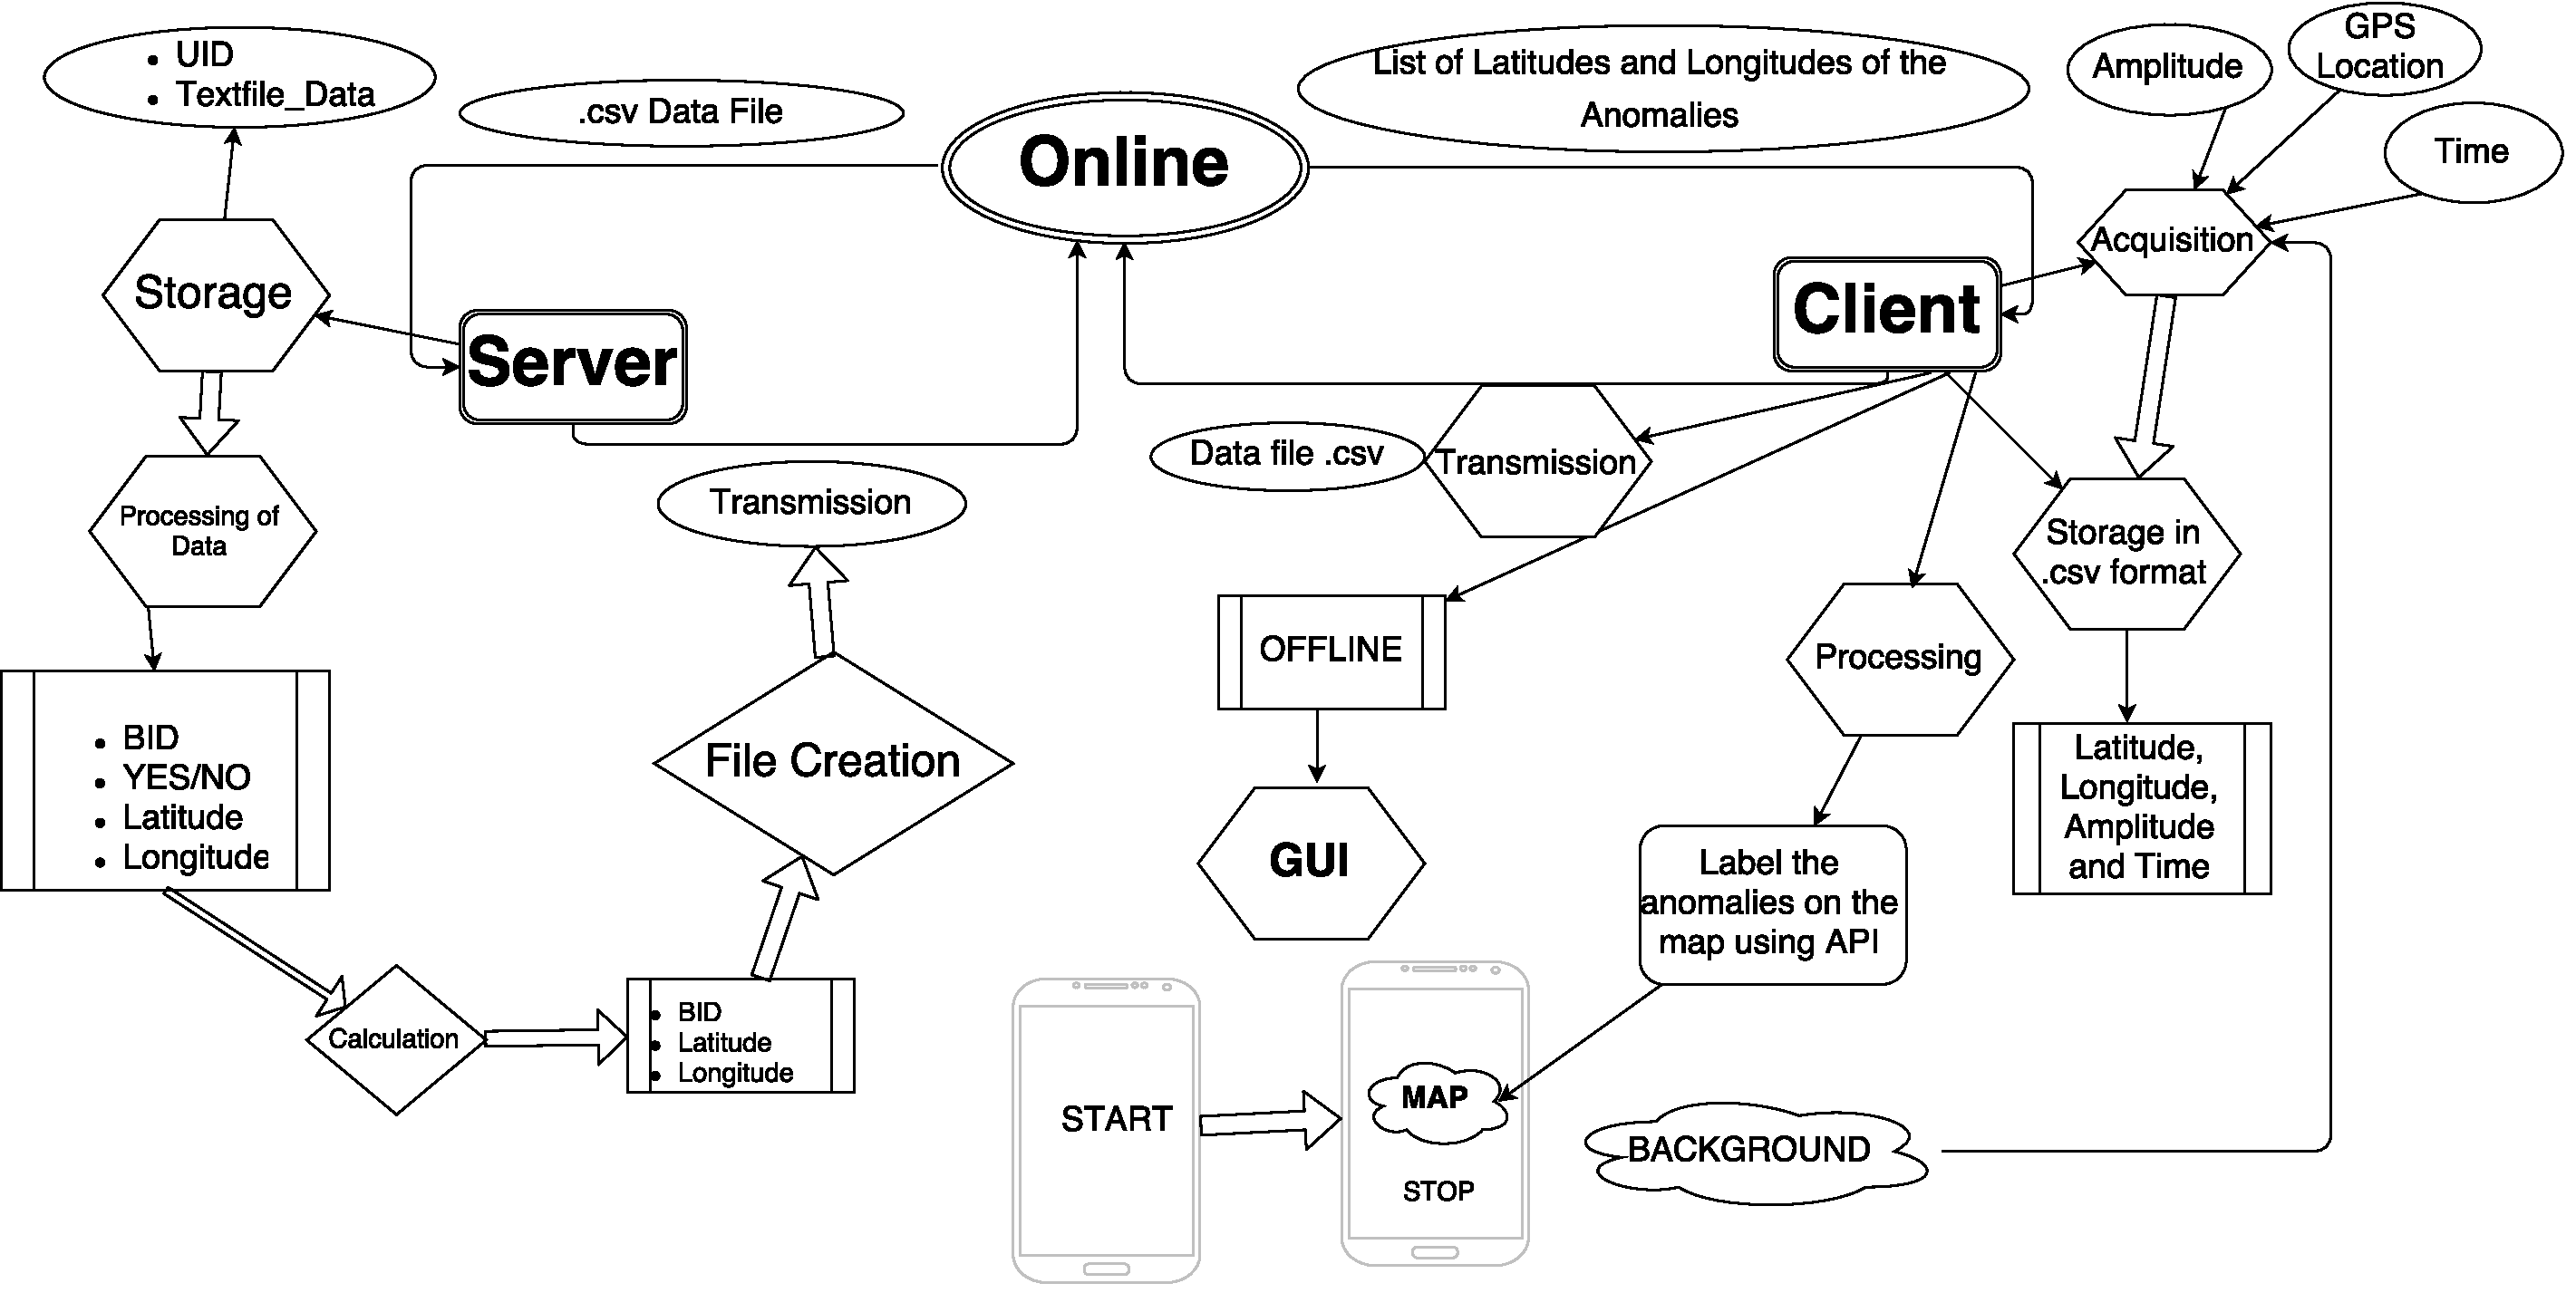
\includegraphics[width= 120mm,height=80mm]{final1_block.jpg}
\end{figure} 
\begin{figure}[ht!]
\centering
\includegraphics[width= 120mm,height=80mm]{choubey.jpg}
\end{figure} 
\newpage
\textbf{Tools Used :}
\begin{enumerate}
\item Android file upload to the server (HttpURLConnection of Android for communication with the server and file upload using the HTTP multi-part/form-data protocol for file uploads).
\item Server is built with Django framework
\item Server side handling of the request for the speed breakers form the android clients (Django rest framework ).
\item Managing of asynchronous task of file analyzing in the background (Celery using Reddit queue).
\item Database management (PostgreSQL implemented with python using psycopg)
\item Octave
\item FOR GPS:android.location package 
\item FOR ACCELEROMETER:android.harware.SensorEvent	 					package
\item FOR MAPS:Google Maps Android API\\
\end{enumerate}
\textbf{Results}\\
At server each client is now capable of generating a file with any road anomaly and its corresponding GPS coordinates.
An application is created which when active takes reading of the x,y and z axes of the accelerometer of the smart-phone along with the GPS coordinates when active.
The application will guide through a visible map on screen. It is capable of receiving data from the server and plotting the anomalies(which matter) on the screen.
The server also analyses the data sent by the client and finds out the road anomalies and their corresponding time and GPS coordinates. This data is saved to a database.
We plot the amplitude against time for a given set of readings. Which looks like the graph below. Here the peak shows the existence of speed breaker at the given time.
\begin{figure}[ht!]
\centering
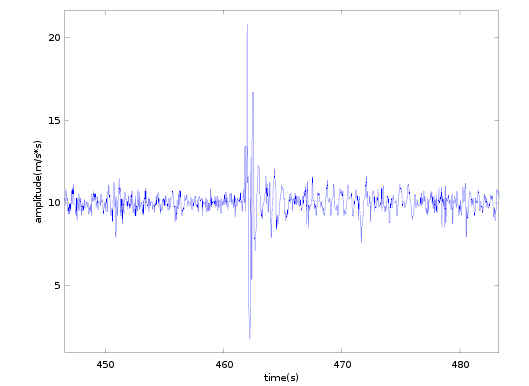
\includegraphics[width= 120mm,height=80mm]{sc1.png}
\end{figure} 
\newpage
The spectrogram of the following data looks like this.
\begin{figure}[ht!]
\centering
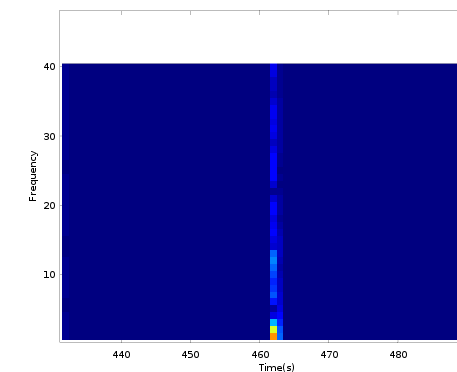
\includegraphics[width= 120mm,height=80mm]{sc1-1.png}
\end{figure} 
\newpage
From spectrogram of the data we can easily compute the time at which speed breaker occurs. Here these two figures above show how time of the speed breaker can be computed. First figure tells that around 462 seconds the breaker exists. Second figure which is the spectrogram of the same data which we plot in the previous figure confirms by showing different color pattern at time 462.
From the following observations we can compute the time when speed-breaker exists and we keep the track of latitude and longitude corresponding to that time.\\
\textbf{Future Work}\\
We were able to detect and warn early about the speed-breakers. In the future this topic interests us to work upon a wider set of road anomalies. Who knows that the advancement in technology drives us to what? Maybe one day we will teleport or something. Clearly that day is far away.
We can work on an off road tracker. A system which detects whether you are going on a road or how likely you are to getting away from it. It'll monitor whether you are awake and attentive or not. Maybe it will tell you to take a break from driving in once in a while.
Face detection and image detection would contribute to this idea as well. We could detect the eyes of the driver and even the obstructions on the road to assist the driver in any way possible.
If the application is deployed and is a success. Consider that all the vehicles on the road have it, we can predict about how good is it for you to overtake the vehicle in front of you.
If the user witnesses an accident, the concerned authorities would need to know immediately, the application will further contain an emergency button to make the driver feel more secure.
The system will keep in account of the time of the day (nights tend to be more accident prone) and the weather (rainy, snowy etc). This way according to different situations the system will produce appropriate speed warnings and alarms.
Further the application created could be power efficient. It would keep in account the power consumption of various sensors. Sure you wouldn't want your phone to run out of juice while assisting you with your route.
The field is wide. And we would like to explore further. We can also introduce auditory alarms for the fore coming anomalies. This way you wouldn't have to keep staring at the screen and drive more comfortably.\\
\textbf{Conclusions}\\
So with the help of the resources and after some time we were able to build a Driving Assistance system using an Android Smart-phone. You can get the warnings of all the breakers on the road you are traveling. It will use minimum amount of mobile data. Moreover you are also reporting about the breakers you came across. So next time you go to your office, we will remind you where your breaker lies.
With further advancement we will be able to include suited auditory alerts for the breakers.
With time we shall be able to deploy it successfully and help prevent some major or minor accidents. We only hope to make your journey smooth. Thank you for bearing with us.\\
\textbf{References}\newline
[1]	Speed-breaker Early Warning system,Mohit Jain, Ajeet Pal Singh ,JIIT, Noida, India ; 	Soshant Bali, Sanjit Kaul IIIT-D, New Delhi, India \newline
[2]	FUNDAMENTAL CONCEPTS \& AN OVERVIEW OF THE WAVELET THEORY 
	Second Edition June 5,1996 ,Robi Polikar\newline
[3]	Pothole Detection Using Machine Learning Aniket Kulkarni, 	Nitish Mhalgi, Sagar 	Gurnani, Dr. Nupur Giri,International 	Journal of Emerging Technology and Advanced 	Engineering Volume 4, Issue 7, July 2014\newline
[4]	Google driver-less car : https://en.wikipedia.org/wiki/Google\_driverless\_car\newline
[5]	Shubhangi Pargaonkar, Diksha Jawalkar, Reshma Chate ,Shivani Sangle ,M.D.Umale, 	S.S.Awate "Safe 	Driving Using Android Based Device ", International Journal of 	Engineering Trends and Technology (IJETT), 	V18(3),151-154 Dec 2014. ISSN:2231-	5381. www.ijettjournal.org. published by seventh sense research group \newline

\end{document}
